\newpage
\begin{appendices}
\appendixpage
\noappendicestocpagenum
\addappheadtotoc
\addcontentsline{toc}{chapter}{\appendixname}

\chapter{Bird Daemon's Configuration using v0.3 Package - UOC's VM in Guifi.net}
\label{app:ch:bdcuoc}

\section{UCI Configuration}
\begin{lstlisting}[language=bash,caption={UCI Configuration}]
config bird 'bird'
        option use_UCI_config '1'
        option UCI_config_file '/tmp/bird4.conf'
        option UCI_config_File '/tmp/bird4.conf'

config global 'global'
        option log_file '/tmp/bird4.log'
        option router_id '10.139.173.161'
        option log 'all'

config table
        option name 'aux'

config kernel 'kernel1'
        option import 'all'
        option export 'all'
        option scan_time '10'
        option learn '1'
        option disabled '0'

config device 'device1'
        option scan_time '10'
        option disabled '0'

config bgp_template 'BGP_COMMON'
        option receive_limit_action 'warn'
        option local_as '92099'
        option igp_table 'bgpTable'
        option export_limit_action 'warn'
        option import_limit_action 'warn'
        option next_hop_self '0'
        option next_hop_keep '0'
        option rr_client '0'

config table
        option name 'bgpTable'

config bgp 'BGPImportALL'
        option receive_limit_action 'warn'
        option template 'BGP_COMMON'
        option neighbor_as '59361'
        option neighbor_address '172.25.35.25'
        option export_limit_action 'warn'
        option import_limit_action 'warn'
        option import_limit '3000'
        option import 'filter ebgp_in'
        option export 'filter ebgp_out'
        option next_hop_self '0'

config kernel 'Kernel_BGP'
        option disabled '0'
        option table 'bgpTable'
        option kernel_table '251'
        option scan_time '10'
        option learn '1'
        option import 'all'
        option export 'all'

config pipe 'pipe1'
        option disabled '0'
        option peer_table 'bgpTable'
        option table 'aux'
        option import 'all'
        option export 'all'
        option mode 'transparent'

config direct 'direct1'
        option disabled '0'
        option interface '"br-lan","br-wan", "br-mgmt"'

config static 'static1'
        option disabled '0'
        option table 'aux'
\end{lstlisting}

\section{Bird Configuration}
\begin{lstlisting}[language=bash,caption={Bird4.conf Configuration}]
#Bird4 configuration using UCI:

log "/tmp/bird4.log" all;

#Router ID
router id 10.139.173.161;

#Secondary tables
table aux;
table bgpTable;

#Functions Section:
include "/etc/bird4/functions/function-20170507-1038";
#End of Functions --

#Filters Section:
include "/etc/bird4/filters/filter-20170507-0951";
#End of Filters --

#kernel1 configuration:
protocol kernel kernel1 {
#   disabled;
    learn;
    persist;
    scan time 10;
    import all;
    export all;
}

#Kernel_BGP configuration:
protocol kernel Kernel_BGP {
#   disabled;
    table bgpTable;
    kernel table 251;
    learn;
    persist;
    scan time 10;
    import all;
    export all;
}

#static1 configration:
protocol static {
    table aux;
}

#device1 configuration:
protocol device {
#   disabled;
    scan time 10;
}

#direct1 configuration:
protocol direct {
#   disabled;
    interface "br-lan","br-wan", "br-mgmt";
}

#pipe1 configuration:
protocol pipe pipe1 {
#   disabled;
    table aux;
    peer table bgpTable;
    mode transparent;
    import all;
    export all;
}

#BGP_COMMON template:
template bgp BGP_COMMON {
    local as 92099;
#    next hop self;
#    next hop keep;
    igp table bgpTable;
#    rr client;
}

#BGPImportALL configuration:
protocol bgp BGPImportALL from BGP_COMMON {
    import filter ebgp_in;
    export filter ebgp_out;
#    rr client;
    import limit 3000 action warn;
    neighbor 172.25.35.25 as 59361;
}

========================================
BGP Filters and Functions:
root@LEDE-eloi:~# cat /etc/bird4/filters/filter-20170507-0951
filter ebgp_in {

        krt_prefsrc = 10.139.173.161;

        if match_guifi_prefix() then accept;
        reject;
}

filter ebgp_out {

        if match_guifi_prefix() then accept;
        reject;
        

root@LEDE-eloi:~# cat /etc/bird4/functions/function-20170507-1038
function match_guifi_prefix()
{
        return net ~ [ 10.0.0.0/8{9,32} ];
}
\end{lstlisting}


\chapter{Bird Daemon presence in Worldwide IXPs and other institutions}
\label{app:ch:blinks}

\chapter{Kanban Project Management using Taiga.io Service}
\label{app:sec:kanban}
As part of the initial investigation, I did some research on Open Source Project Management tools that could help me monitoring my progress as well as adding some value to the final project.
Because of this project's scope and time-frame, the size of the team (me) and the number of Stakeholders (Víctor), the only Agile \textit{approach} that I could use was Kanban\footnote{\href{http://www.scrumhub.com/kanban-fundamentals/}{Kanban} approach summarised: project with a continuous prioritised backlog, one task per team resource, the project must be releasable after closing any task, reduce to the minimum the number of required ceremonies and tasks go from \textit{ToDo} (left) to \textit{Done} (right).}. The following sections present the tests and initial usage of Taiga Kanban service.

\begin{landscape}
\section{EPICS View}
\begin{figure}[h!]
\centering
    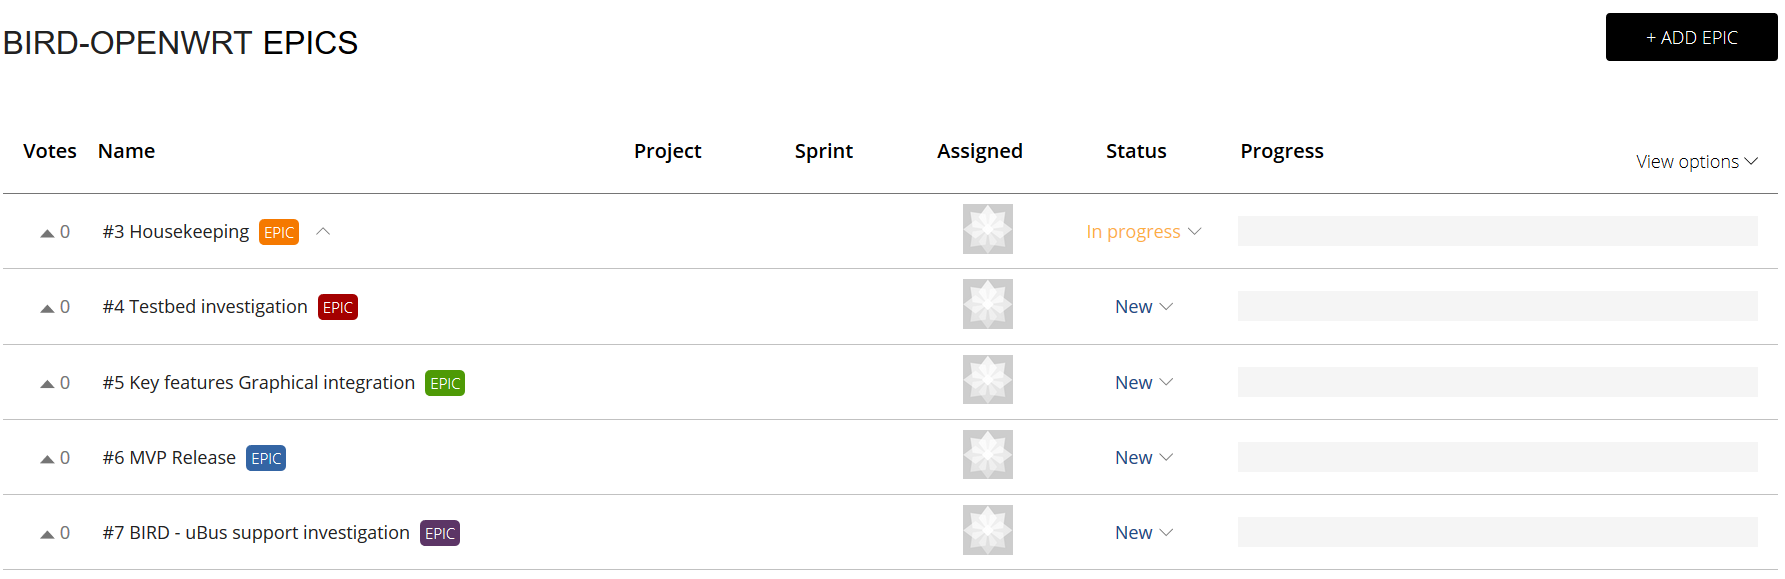
\includegraphics[width=\hsize]{images/kanban/epics}
    \caption{Project EPICs overview}
    \label{fig:kepic}
\end{figure}

This view presents the information about the big tasks represented in project's schedule, who is working on each one, other useful information and how far it is the task of being delivered.
\newpage

\subsection{EPIC Detail View}
\begin{figure}[h!]
\centering
    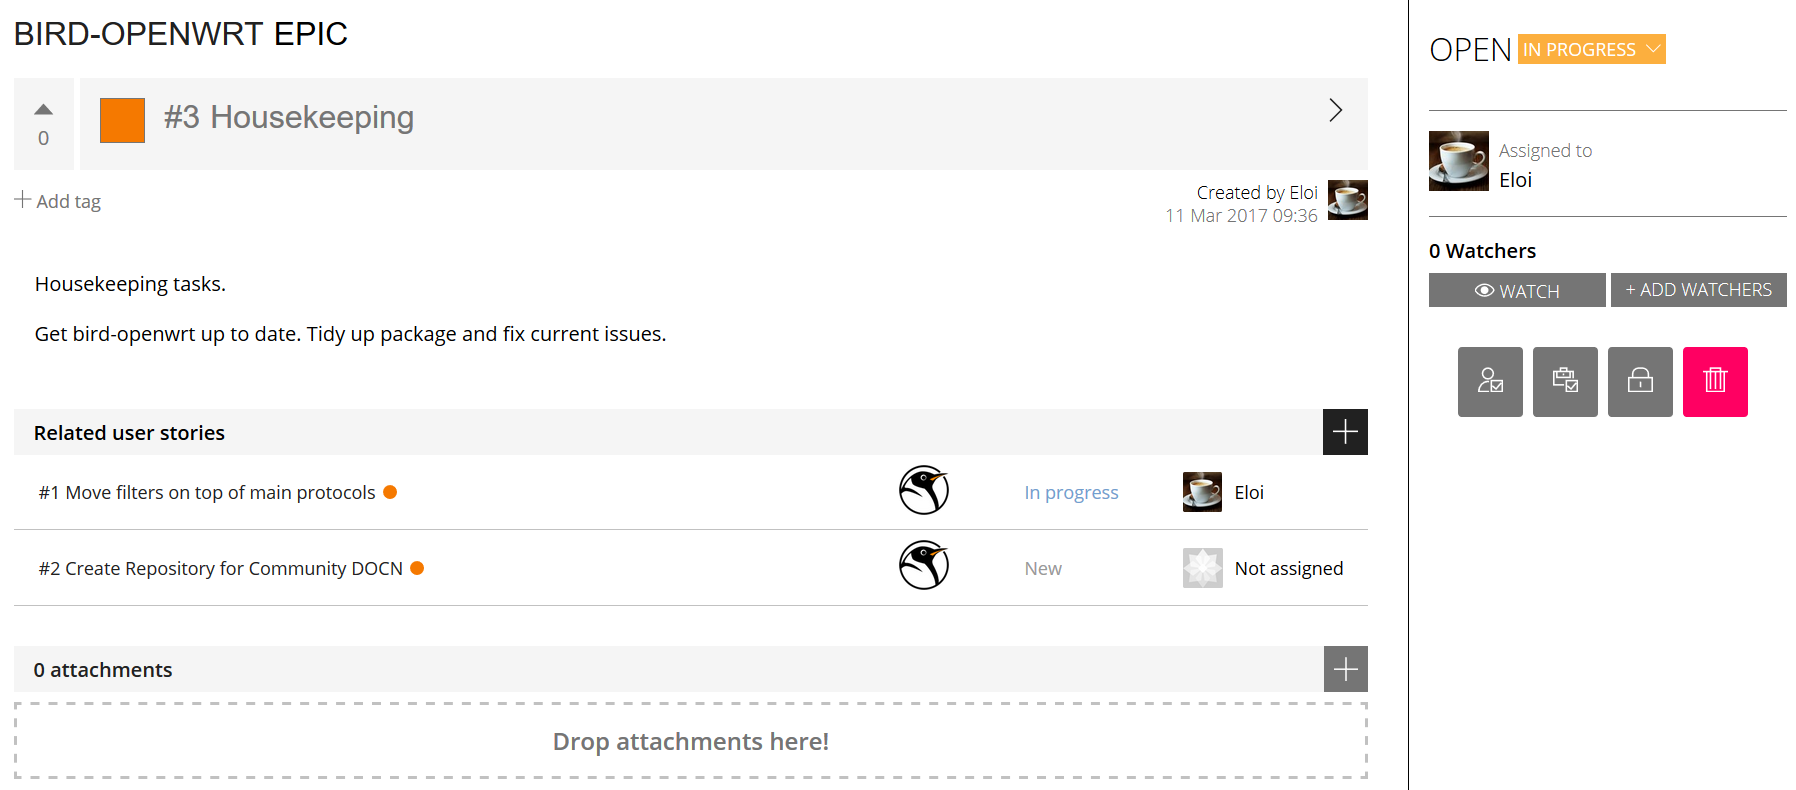
\includegraphics[width=0.85\hsize]{images/kanban/epic-details}
    \caption{Housekeeping EPIC detailed view}
    \label{fig:kepicd}
\end{figure}
This view presents the detailed information of a specific Epic. It presents the first EPIC \textit{Housekeeping} which is In Progress, assigned to \textbf{Eloi} and two tasks, one already in progress and another waiting for resources.
\newpage

\section{Timeline View}
\begin{figure}[h!]
\centering
    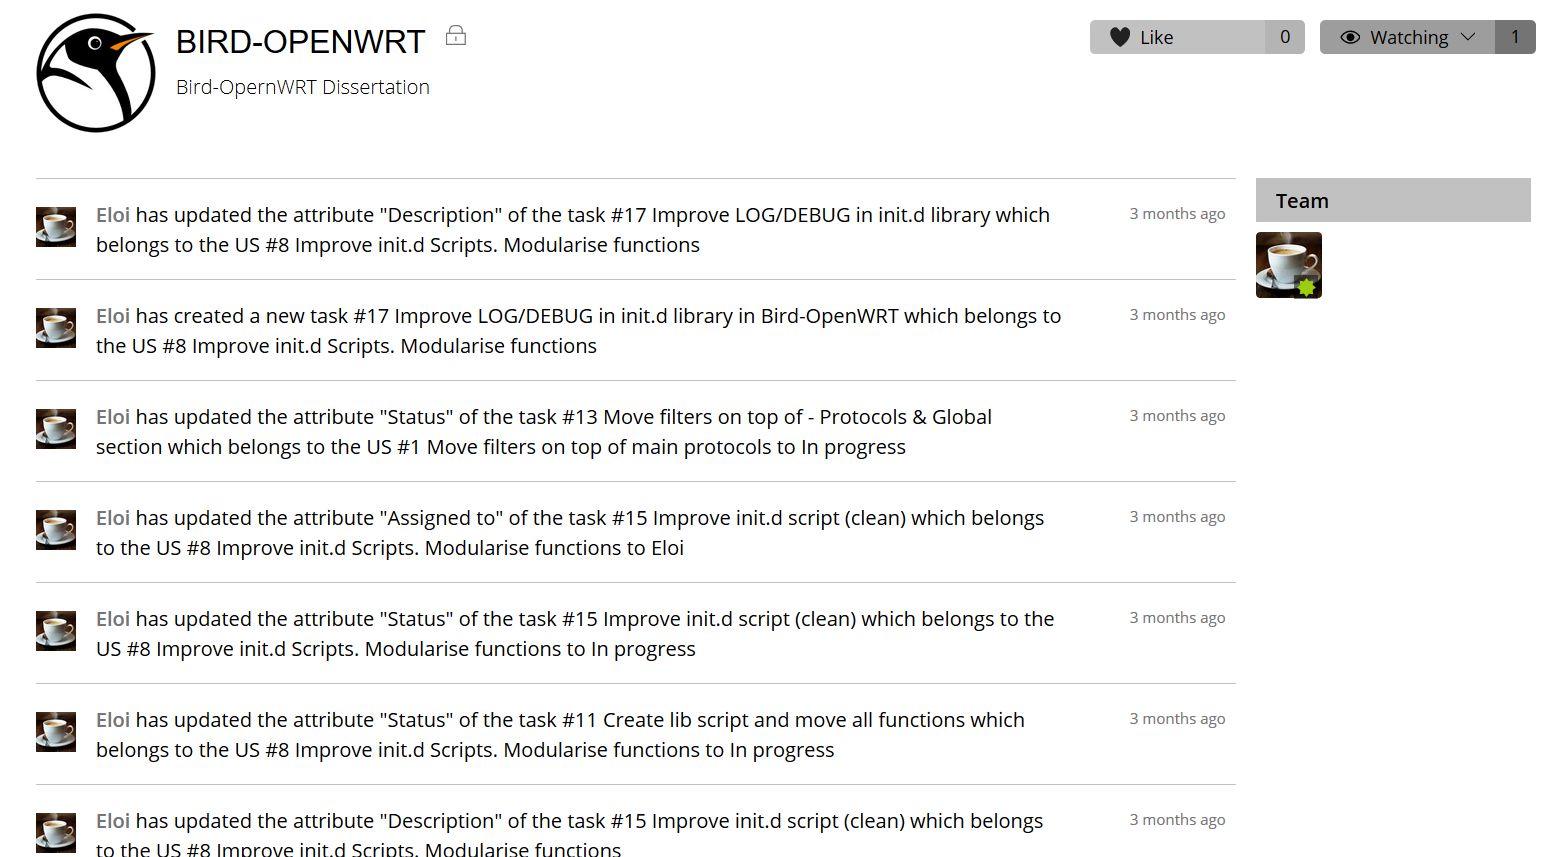
\includegraphics[width=0.7\hsize]{images/kanban/timeline}
    \caption{Project timeline status information}
    \label{fig:ktimeline}
\end{figure}
The Timeline View presents Project's log information. Any action applied to any of the tasks, stories or epics will be logged and shown chronologically in this page.
\newpage

\section{Kanban Board View}
\begin{figure}[ht!]
\centering
    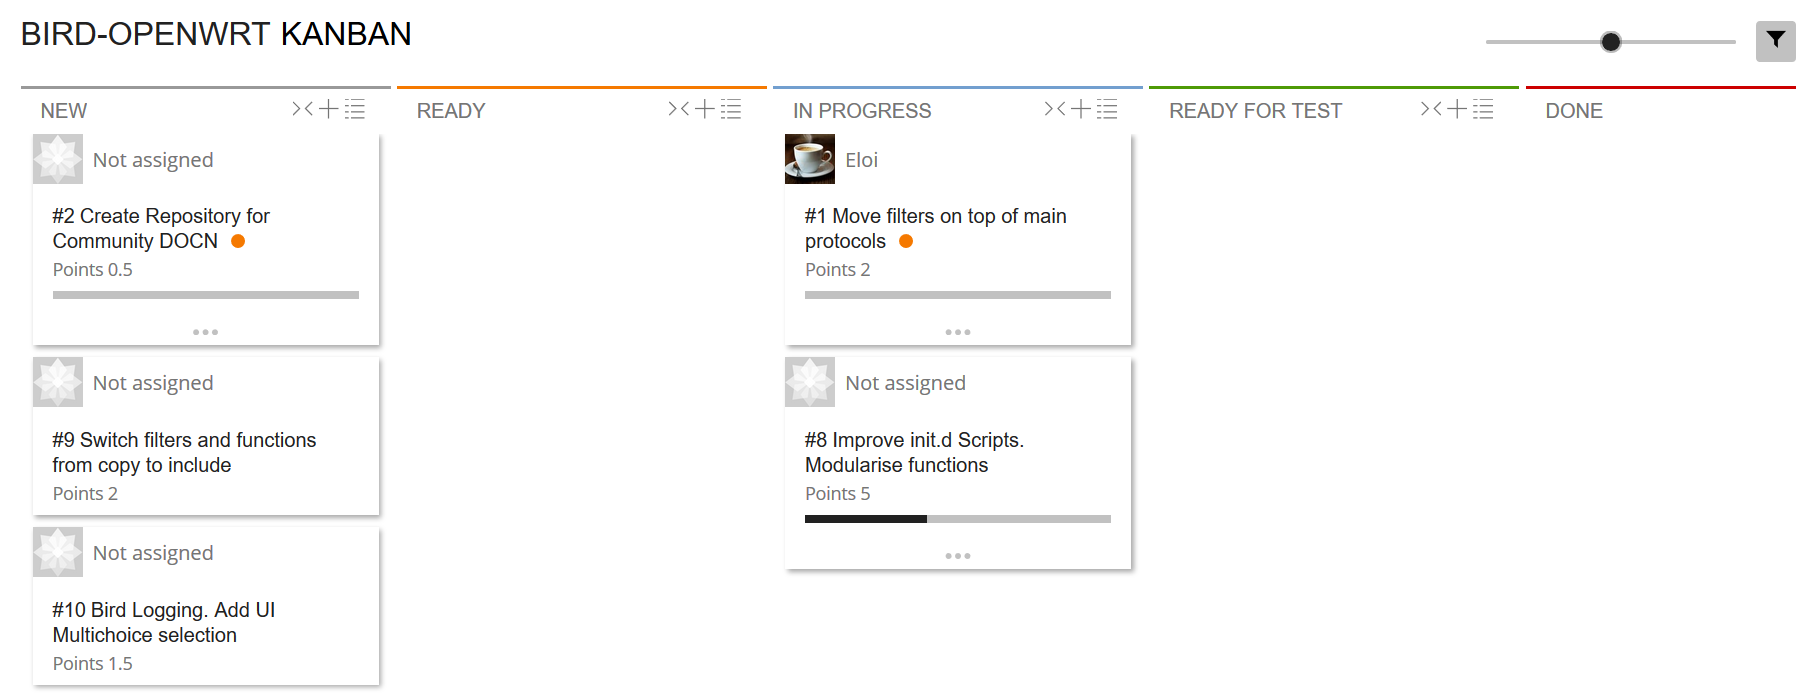
\includegraphics[width=0.85\hsize]{images/kanban/kanban}
    \caption{Kanban User Stories board view}
    \label{fig:kboard}
\end{figure}
The Kanban Board shows the state of the User Stories being addressed, in which state and how far they are from being completed.
\newpage

\subsection{Cycle/Sprint View}
\begin{figure}[ht!]
\centering
    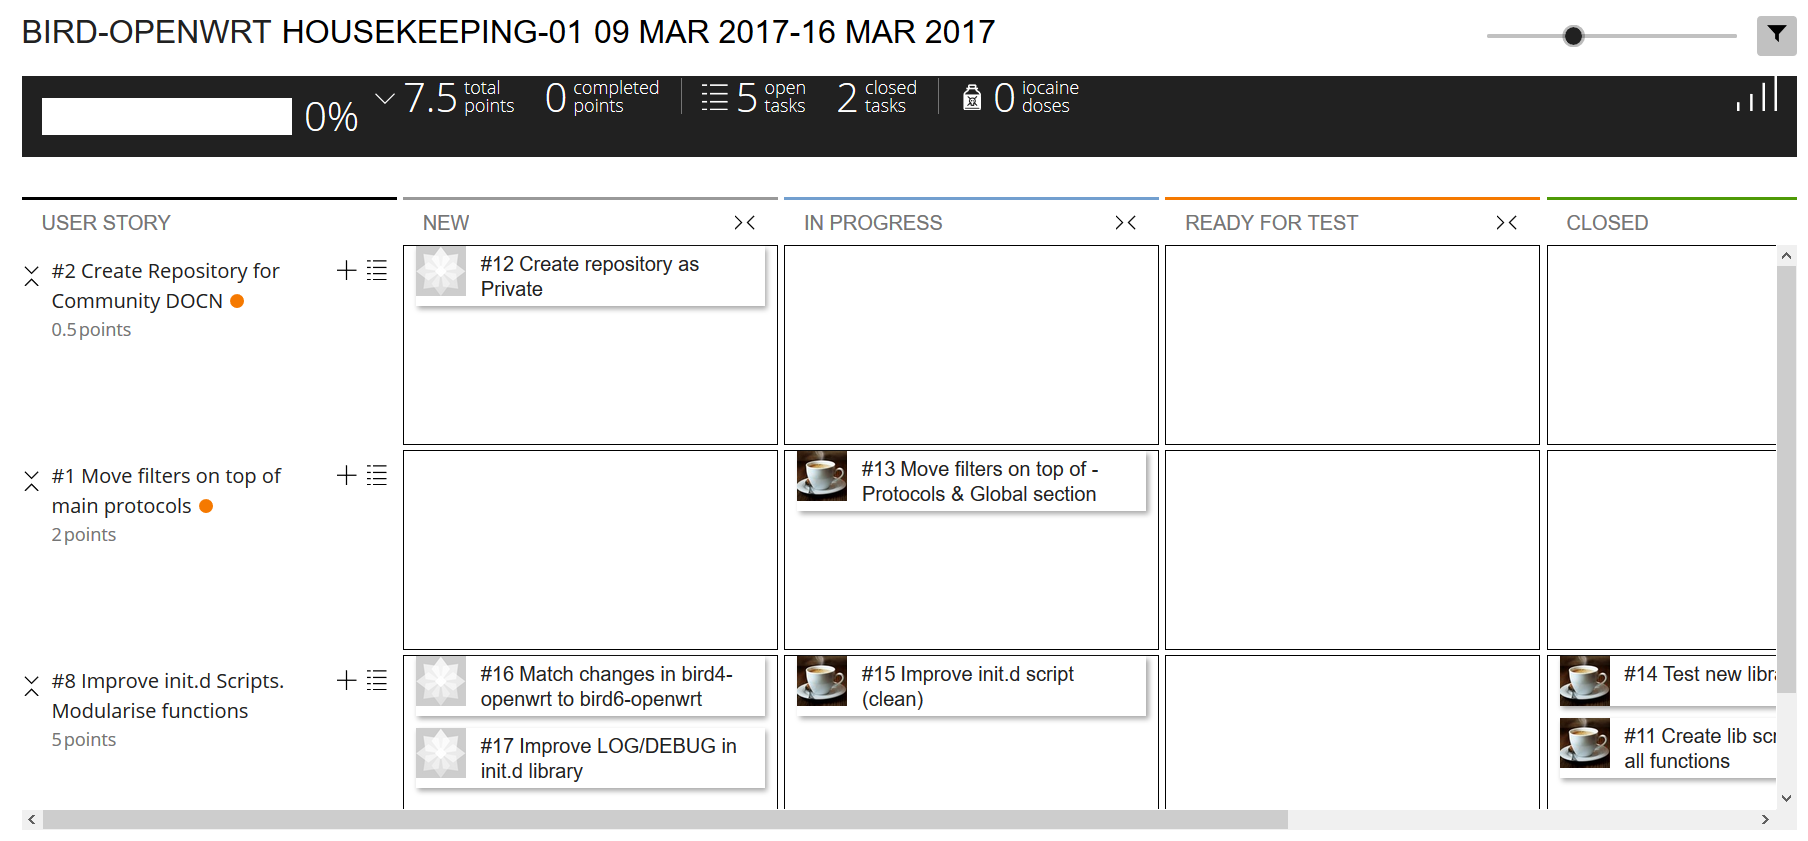
\includegraphics[width=0.85\hsize]{images/kanban/cycle}
    \caption{Kanban current cycle/sprint tasks board view}
    \label{fig:kcycle}
\end{figure}
The Cycle/Sprint View presents the user stories being addressed in priority order (in the left) and all the involved Tasks required to complete each of these user stories, to who are assigned and their state. This is a detailed view of the Kanban Board View.

\end{landscape}

\chapter{Extra LUCI Example Pages}
\label{app:ch:extrap}

\section{Privoxy LUCI2 Status Page}
\begin{figure}[H]
    \centering
    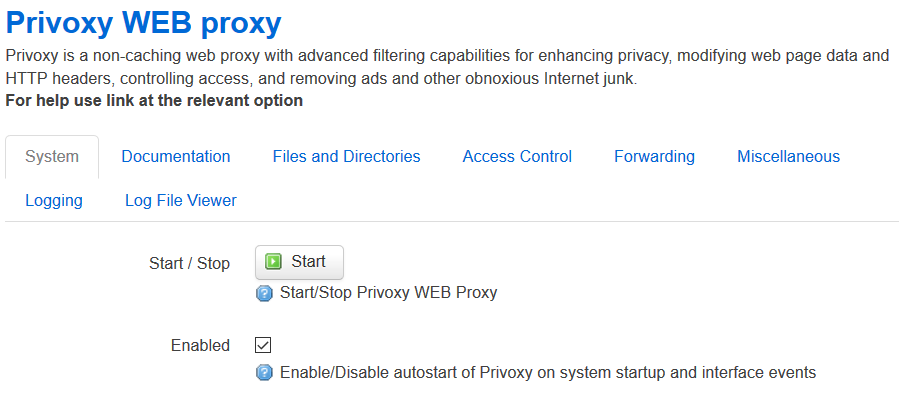
\includegraphics[width=0.95\textwidth]{images/luciextra/disabled}
    \caption{Privoxy \textbf{disabled} service.}
    \label{fig:privdis}
\end{figure}

\begin{figure}[H]
    \centering
    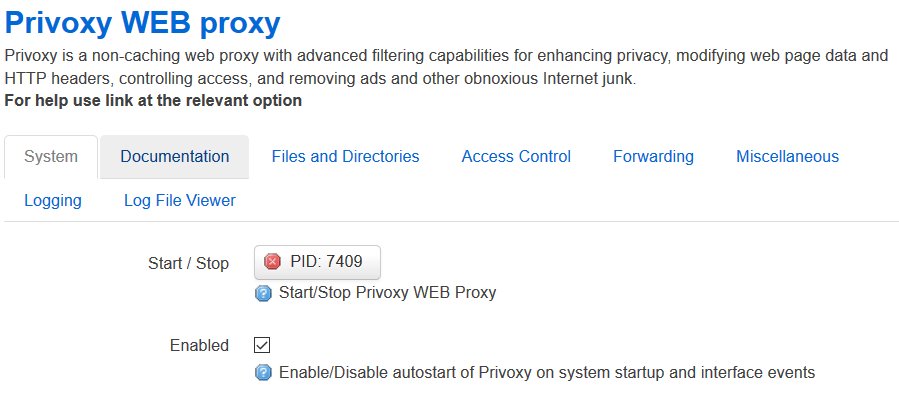
\includegraphics[width=0.95\textwidth]{images/luciextra/enabled}
    \caption{Privoxy \textbf{enabled} service.}
    \label{fig:priven}
\end{figure}
\end{appendices}